\chapter{OTA - Exercício 5} \label{Chap:AppendixTangente}


\begin{xltabular}{\textwidth}{|l|X|}
	\hline
	\endfirsthead
	
	\hline \multicolumn{2}{|c|}{continuação da página anterior} \\ \hline
	\endhead
	
	\hline \multicolumn{2}{|r|}{Continua na próxima página} \\ \hline
	\endfoot
	
	\hline
	\endlastfoot
	
	\multicolumn{2}{|c|}{\cellcolor[HTML]{C0C0C0}\textbf{ASPECTOS EDUCACIONAIS}} \\ \hline
	\textbf{NOME} & Quadro Trigonométrico - Tangente\\ \hline
	\textbf{DESCRIÇÃO GERAL} & Este objeto de aprendizagem trabalha com conceitos relacionados a Trigonometria, em especial, valores e posições dos ângulos no círculo trigonométrico.\\ \hline
	\textbf{TÓPICOS} & Trigonometria, ângulos, círculo trigonométrico, quadrantes, graus, radianos\\ \hline
	\textbf{DESCRIÇÃO EDUCACIONAL} & No Player Virtual, o estudante deve escolher o ângulo que irá estudar e, então, deve manipular o ponteiro do objeto físico (Player Físico) de modo a indicar a posição deste ângulo. O ponteiro virtual é movimentado a partir da manipulação do ponteiro físico e, após a confirmação da posição pelo estudante, é habilitada uma caixa de texto, onde deverão ser inseridos os valores do ângulo em graus e em radianos. Caso o aluno posicione o ponteiro físico em um local que não é a posição correta, ou insira um valor incorreto, o Player Virtual deverá retornar uma informação que ajude o estudante a corrigir os valores ou posições. Este objeto utiliza a Face A05 do OFVA Quadro Trigonométrico. \\ \hline
	\textbf{MODO} & ESTUDO \\ \hline
	\multicolumn{2}{|c|}{\cellcolor[HTML]{C0C0C0}\textbf{DISPOSITIVOS}} \\ \hline
	\textbf{ITENS} & 32 sensores de efeito hall; 1 imã de neodímio; ESP-WROOM-32; 1 Teclado membrana matricial; 1 Display LCD, Interface Wifi \\ \hline
	\multicolumn{2}{|c|}{\cellcolor[HTML]{C0C0C0}\textbf{RECURSOS}} \\ \hline
	\textbf{RECURSOS FÍSICOS} & .hex e .ino em Arduíno, Ponteiro físico, Face A05 com círculo trigonométrico apenas com valores de ângulos estudados em A02 e reta das tangentes.  \\ \hline
	\textbf{RECURSOS DIGITAIS} & Player Virtual \\ \hline		
	\multicolumn{2}{|c|}{\cellcolor[HTML]{C0C0C0}\textbf{SERVIÇOS}} \\ \hline
	\textbf{ITENS} & Iniciar atividade (botão), Leitura de hipertexto, Envio de resposta física (formato: websocket + json + botão físico), Envio de resposta digital (html tracking), Confirmação de resposta (visualização de respostas dadas), Feedback (modo estudo), Encerrar atividade (botão)  \\ \hline
	
\end{xltabular}

\begin{xltabular}{\textwidth}{|c|c|c|c|c|c|}
	\hline
	\endfirsthead
	
	\hline \multicolumn{6}{|c|}{continuação da página anterior} \\ \hline
	\endhead
	
	\hline \multicolumn{6}{|r|}{Continua na próxima página} \\ \hline
	\endfoot
	
	\hline
	\endlastfoot
	
	\multicolumn{6}{|c|}{\cellcolor[HTML]{C0C0C0}\textbf{ENTRADAS E SAÍDAS}} \\ \hline
	\multicolumn{6}{|c|}{\cellcolor[HTML]{DEDEDE}\textbf{CONJUNTO DE ENTRADAS}} \\ \hline
	\textbf{ID} & \textbf{FONTE} & \textbf{RÓTULO} & \textbf{TIPO DE DADO} & \textbf{BLOCOS} & \textbf{JavaScript} \\ \hline
	1 & Físico & EF1 & inteiro & \multicolumn{1}{|l|}{\begin{tabular}[c]{@{}l@{}} \\ 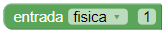
\includegraphics[width=0.2\linewidth]{chapters/appendixSeno/EF1.png}  \end{tabular} } & var EF1; \\ \hline
	2 & Virtual & EV1 & inteiro & \multicolumn{1}{|l|}{\begin{tabular}[c]{@{}l@{}} \\ 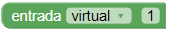
\includegraphics[width=0.2\linewidth]{chapters/appendixSeno/EV1.png}  \end{tabular} } & var EV1; \\ \hline
	3 & Virtual & EV2 & inteiro & \multicolumn{1}{|l|}{\begin{tabular}[c]{@{}l@{}} \\ 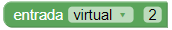
\includegraphics[width=0.2\linewidth]{chapters/appendixSeno/EV2.png}  \end{tabular} } & var EV2; \\ \hline
	4 & Virtual & EV3 & inteiro & \multicolumn{1}{|l|}{\begin{tabular}[c]{@{}l@{}} \\ 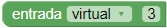
\includegraphics[width=0.2\linewidth]{chapters/appendixSeno/EV3.png}  \end{tabular} } & var EV3; \\ \hline
	5 & Virtual & EV4 & inteiro & \multicolumn{1}{|l|}{\begin{tabular}[c]{@{}l@{}} \\ 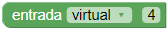
\includegraphics[width=0.2\linewidth]{chapters/appendixSeno/EV4.png}  \end{tabular} } & var EV4; \\ \hline
	6 & Virtual & EV5 & inteiro & \multicolumn{1}{|l|}{\begin{tabular}[c]{@{}l@{}} \\ 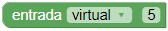
\includegraphics[width=0.2\linewidth]{chapters/appendixSeno/EV5.png}  \end{tabular} } & var EV5; \\ \hline		
	\multicolumn{6}{|c|}{\cellcolor[HTML]{DEDEDE}\textbf{CONJUNTO DE SAÍDAS}} \\ \hline
	\textbf{ID} & \textbf{FONTE} & \textbf{RÓTULO} & \textbf{TIPO DE DADO} &  \multicolumn{2}{|c|}{\textbf{CONTEÚDO}} \\ \hline
	1 & Virtual & SV1 & String & \multicolumn{2}{|l|}{Mova o ponteiro no sentido horário} \\ \hline
	2 & Virtual & SV2 & String & \multicolumn{2}{|l|}{Mova o ponteiro no sentido anti-horário} \\ \hline
	3 & Virtual & SV3 & String & \multicolumn{2}{|l|}{Posição está correta!} \\ \hline
	4 & Virtual & SV4 & String & \multicolumn{2}{|l|}{Resposta está correta!} \\ \hline	
	5 & Virtual & SV5 & String & \multicolumn{2}{|l|}{\begin{tabular}[c]{@{}l@{}} Alguma das respostas precisa ser revista! \end{tabular}} \\ \hline
	%	6 & Virtual & SV5 & String & \multicolumn{2}{|l|}{\begin{tabular}[c]{@{}l@{}} Tente novamente! \end{tabular}} \\ \hline
	\multicolumn{6}{|c|}{\textbf{BLOCOS}} \\ \hline
	\multicolumn{6}{|c|}{\begin{tabular}[c]{@{}l@{}} \\ 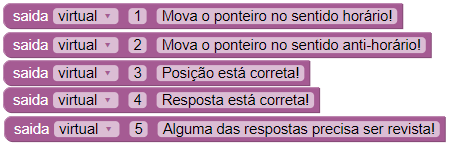
\includegraphics[width=0.6\linewidth]{chapters/appendixSeno/saidas.png}  \end{tabular}} \\ \hline
	\multicolumn{6}{|c|}{\textbf{JavaScript gerado}} \\ \hline
	\multicolumn{6}{|l|}{\begin{tabular}[c]{@{}l@{}} var SV1 = "Mova o ponteiro no sentido horário!";\\ 			var SV2 = "Mova o ponteiro no sentido anti-horário!";\\ 			var SV3 = "Posição está correta!";\\ 			var SV4 = "Resposta está correta!";
			\\			var SV5 = "Alguma das respostas precisa ser revista!";\end{tabular}} \\ \hline
	
\end{xltabular}


\begin{xltabular}{\textwidth}{|l|X|X|}
	\hline
	\endfirsthead
	
	\hline \multicolumn{3}{|c|}{continuação da página anterior} \\ \hline
	\endhead
	
	\hline \multicolumn{3}{|r|}{Continua na próxima página} \\ \hline
	\endfoot
	
	\hline
	\endlastfoot
	
	\multicolumn{3}{|c|}{\cellcolor[HTML]{C0C0C0}\textbf{CASOS DE TESTE}} \\ \hline
	
	%CASO 1
	\multicolumn{3}{|c|}{\cellcolor[HTML]{DEDEDE}\textbf{CASO DE TESTE 1}} \\ \hline
	\multicolumn{1}{|l|}{\textbf{Rótulo:}} & \multicolumn{2}{|l|}{Observar ponteiro}\\ \hline
	\textbf{Situação-problema (Enunciado):} & \multicolumn{2}{|l|}{\begin{tabular}[c]{@{}l@{}} Movimente o ponteiro e marque as alternativas que\\ correspondem às suas observações. 
			
			\\- A reta das tangentes é perpendicular ao eixo y [1]

			\\- A reta das tangentes é paralela ao eixo y [4]
			
			\\- Há ângulos que não possuem tangente. [4] 	
			
			\\- Assim como seno e cosseno, a tangente está limitada \\ao tamanho do círculo. [1]	
			
			\\- Diferente do seno e cosseno, a tangente é uma \\função crescente, ou seja, não há intervalos de \\decrescimento [4]
			
	\end{tabular} }\\ \hline
	\multicolumn{3}{|c|}{\cellcolor[HTML]{DEDEDE}\textbf{REGRA 1}} \\ \hline
	\multicolumn{3}{|c|}{\textbf{Blocos}} \\ \hline
	\multicolumn{3}{|l|}{\begin{tabular}[c]{@{}l@{}} \\ 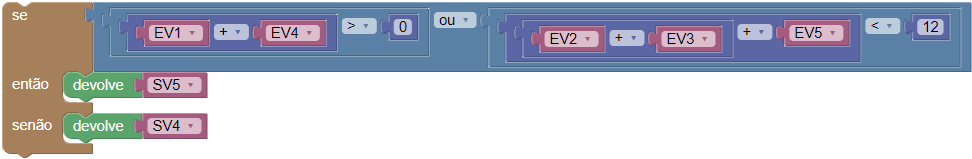
\includegraphics[width=0.9\linewidth]{chapters/appendixTangente/c1r1.png}  \end{tabular}
	} \\ \hline
	\multicolumn{3}{|c|}{\textbf{JavaScript gerado}} \\ \hline
	\multicolumn{3}{|l|}{ \begin{tabular}[c]{@{}l@{}} 
	if ((EV1 + EV4 > 0 || EV2 + EV3 + EV5 < 12))\{   
	\\ \quad return SV5; 
	\\ \}else \{   
	\\ \quad return SV4; 
	\\ \}
	\\ \\ \end{tabular} }\\ \hline
	
	
	%CASO 2
	\multicolumn{3}{|c|}{\cellcolor[HTML]{DEDEDE}\textbf{CASO DE TESTE 2}} \\ \hline
	\multicolumn{1}{|l|}{\textbf{Rótulo:}} & \multicolumn{2}{|l|}{Observar Tangente}\\ \hline
	\textbf{Situação-problema (Enunciado):} & \multicolumn{2}{|l|}{\begin{tabular}[c]{@{}l@{}} Observe o que acontece como valor da tangente, ao \\movimentar o ponteiro para aumentar ou diminuir o valor \\do ângulo, em cada quadrante, e marque as alternativas \\que correspondem às suas observações. 
			
			%Na letra b, a pergunta é direcionada para que os alunos observem e mencionem como se dá a variação dos valores de seno do ângulo, em cada quadrante. Esperamos que além de perceber que o valor do seno aumenta no 1º e no 4º quadrantes e diminui no 2º e 3º quadrantes, os alunos associem os sinais assumidos pelo seno nos respectivos quadrantes.
			
			%	\\1. O valor do seno aumenta no 1º e no 4º quadrantes. 
			%	\\2. o seno do 1º e 2º quadrantes é positivo.
			%	\\3. O valor do seno diminui no 2º e no 3º quadrantes. 
			%	\\4. o seno do 3º e 4º quadrantes é negativo.
			
			\\- O valor da tangente diminui no 2º e aumenta no 1º \\quadrante. [2]
			\\- O valor da tangente aumenta no 3º e no 4º quadrantes.[4]
			\\- A tangente do 2º e 4º quadrantes é negativa. [4]
			\\- A tangente de 90° não existe. [4]
			\\- A tangente do 1º e 4º quadrantes é positiva. [2]
			
	\end{tabular} }\\ \hline
	\multicolumn{3}{|c|}{\cellcolor[HTML]{DEDEDE}\textbf{REGRA 1}} \\ \hline
	\multicolumn{3}{|c|}{\textbf{Blocos}} \\ \hline
	\multicolumn{3}{|l|}{\begin{tabular}[c]{@{}l@{}} \\ 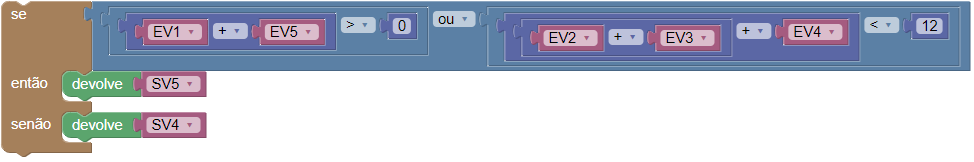
\includegraphics[width=0.9\linewidth]{chapters/appendixTangente/c2r1.png}  \end{tabular}
	} \\ \hline
	\multicolumn{3}{|c|}{\textbf{JavaScript gerado}} \\ \hline
	\multicolumn{3}{|l|}{ \begin{tabular}[c]{@{}l@{}}
	if ((EV1 + EV5 > 0 || EV2 + EV3 + EV4 < 12))\{
	\\ \quad   return SV5; 
	\\ \}else \{   
	\\ \quad return SV4; 
	\\ \}
	\\
	\end{tabular} }\\ \hline
	
	
	%CASO 3
	\multicolumn{3}{|c|}{\cellcolor[HTML]{DEDEDE}\textbf{CASO DE TESTE 3}} \\ \hline
	\multicolumn{1}{|l|}{\textbf{Rótulo:}} & \multicolumn{2}{|l|}{$tan x = 1$}\\ \hline
	\textbf{Situação-problema (Enunciado):} & \multicolumn{2}{|l|}{\begin{tabular}[c]{@{}l@{}} 
			A sentença apresenta um resultado para a tangente de um \\ângulo desconhecido x. Usando o ponteiro físico, \\encontre um valor de x que a satisfaça.\end{tabular} }\\ \hline
	\multicolumn{3}{|c|}{\cellcolor[HTML]{DEDEDE}\textbf{REGRA 1}} \\ \hline
	\multicolumn{3}{|c|}{\textbf{Blocos}}\\ \hline
	\multicolumn{3}{|l|}{\begin{tabular}[c]{@{}l@{}} \\ 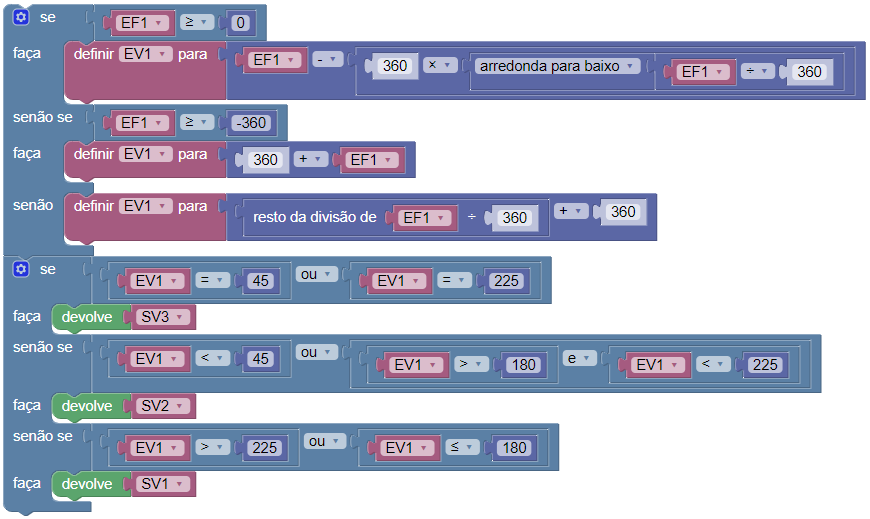
\includegraphics[width=0.9\linewidth]{chapters/appendixTangente/c3r1.png} \\ \end{tabular}
	} \\ \hline
	\multicolumn{3}{|c|}{\textbf{JavaScript gerado}}\\ \hline
	\multicolumn{3}{|l|}{\begin{tabular}[c]{@{}l@{}} 
			
	if (EF1 >= 0) \{
	\\ \quad	EV1 = EF1 - 360 * Math.floor(EF1 / 360);
	\\ \} else if (EF1 >= -360) \{
	\\ \quad	EV1 = 360 + EF1;
	\\ \} else \{
	\\ \quad	EV1 = EF1 \% 360 + 360;
	\\ \}
	if (EV1 == 45 || EV1 == 225) \{
	\\ \quad return SV3;
	\\ \} else if (EV1 < 45 || EV1 > 180 \&\& EV1 < 225) \{
	\\ \quad return SV2;
	\\ \} else if (EV1 > 225 || EV1 <= 180) \{
	\\ \quad return SV1;
	\\ \}			
	\end{tabular} }\\ \hline
	
	
	
	%CASO 4
	\multicolumn{3}{|c|}{\cellcolor[HTML]{DEDEDE}\textbf{CASO DE TESTE 4}} \\ \hline
	\multicolumn{1}{|l|}{\textbf{Rótulo:}} & \multicolumn{2}{|l|}{$tan x = -0,1763...$}\\ \hline
	\textbf{Situação-problema (Enunciado):} & \multicolumn{2}{|l|}{\begin{tabular}[c]{@{}l@{}} 
			A sentença apresenta um resultado para a tangente de um \\ângulo desconhecido x. Usando o ponteiro físico, \\encontre um valor de x que a satisfaça.\end{tabular} }\\ \hline
	\multicolumn{3}{|c|}{\cellcolor[HTML]{DEDEDE}\textbf{REGRA 1}} \\ \hline
	\multicolumn{3}{|c|}{\textbf{Blocos}} \\ \hline
	\multicolumn{3}{|l|}{\begin{tabular}[c]{@{}l@{}} \\ 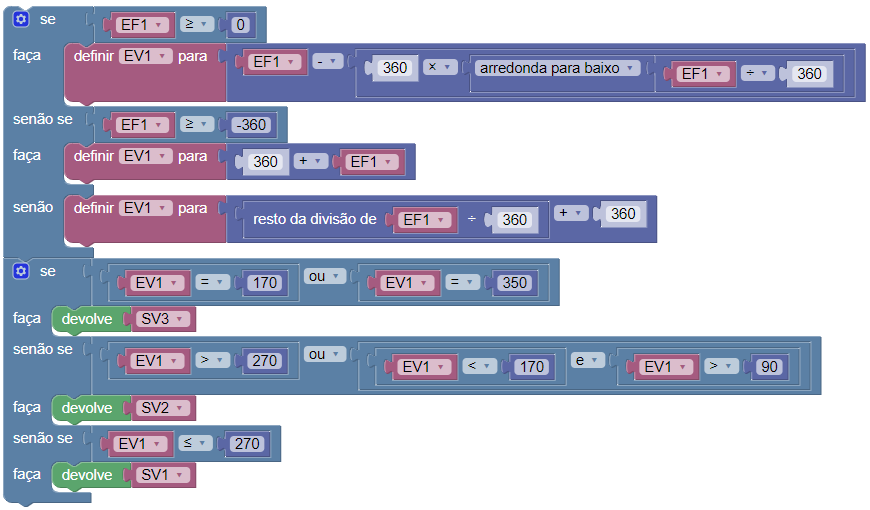
\includegraphics[width=0.9\linewidth]{chapters/appendixTangente/c4r1.png}  \end{tabular} } \\ \hline
	\multicolumn{3}{|c|}{\textbf{JavaScript gerado}} \\ \hline
	\multicolumn{3}{|l|}{ \begin{tabular}[c]{@{}l@{}}
	if (EF1 >= 0) \{
	\\ \quad	EV1 = EF1 - 360 * Math.floor(EF1 / 360);
	\\ \} else if (EF1 >= -360) \{
	\\ \quad	EV1 = 360 + EF1;
	\\ \} else \{
	\\ \quad	EV1 = EF1 \% 360 + 360;
	\\ \}
	if (EV1 == 170 || EV1 == 350) \{
	\\ \quad	return SV3;
	\\ \} else if (EV1 > 270 || EV1 < 170 \&\& EV1 > 90) \{
	\\ \quad	return SV2;
	\\ \} else if (EV1 <= 270) \{
	\\ \quad	return SV1;
	\\ \}
	\end{tabular} }\\ \hline
		
\end{xltabular}